\documentclass[../thesis.tex]{subfiles}
\begin{document}

\chapter{Stock Trading Preliminaries}
\label{ch:prelim}


\section{Stock Trading}
In this study we examine numerous algorithmic trading methods. To measure the effectiveness of a particular strategy, we use a quality metric to analyze productivity. Different denominations of purchasing powers are used and compared against a \textit {buy-and-hold baseline}. The baseline measure is created by holding a long position of a specific denomination throughout the entire period of trading. Simply put, shares are bought at the beginning of the period and sold at the end. The profit level is then compared against the performance of the AT strategy. Much of the literature actively study the best performance of these strategies over different periods and use the same baseline comparison \cite{Liu2006} \cite{Aldridge2010} \cite{Garcia2015}. We therefore include the same baseline in this study.

The stocks used in all strategies are found in Figure~\ref{stocktable}. These stocks were chosen given the availability of NASDAQ and S\&P500 stocks in the Quandl dataset and cover a variety of industries. This is important because we need to account for different performances of stocks. Certain large tech stocks like FB or GOOG have had incredible trajectories and performances whereas other stocks outside of the tech industry like HAS, have performed more moderately. The range of stocks chosen encompass nearly all of the major industries throughout the world.

\textit {Buy} and \textit {sell signals} are used throughout the study. Algorithms can generate a variety of buy and sell signals at a specific point in time, indicating that some denomination of stocks should be purchased or sold at that specific point in time. To measure how a given algorithm performs, different denominations of shares are purchased and compared. The strategies use closing price data from October 1st, 2006 to January 1st, 2017. Some strategies use intra-day stock data, which is minute-by-minute data of stock prices from October 26, 2018. Other additional terms need to be defined. \textit {Securities} and \textit{stocks} are used interchangeably throughout the paper and effectively have the same meaning. Specifically, securities have more of a broad definition, as securities include stocks, bonds, mortgages, and others. When discussing how stocks will move in the future, we use \textit {bearish signals} to signal trends of downturn and \textit {bullish signals} for positive, upward trends \cite{Aldridge2010}. 

Graphs can be interpreted as follows. Figure~\ref{SMAfigure} shows the Simple Moving Average strategy applied to GOOG. Purple triangles, which are angled upwards, are buy signals while black triangles angled downwards are sell signals. On June 2015, the strategy generated a sell signal, denoted by the black triangle. In the following couple of months, a subsequent buy signal was generated as denoted by the purple triangle. The orange line is the long moving average, the blue line is the short moving average, and the red line gives the price of GOOG throughout the time. 

\begin{figure}[h]
\centering
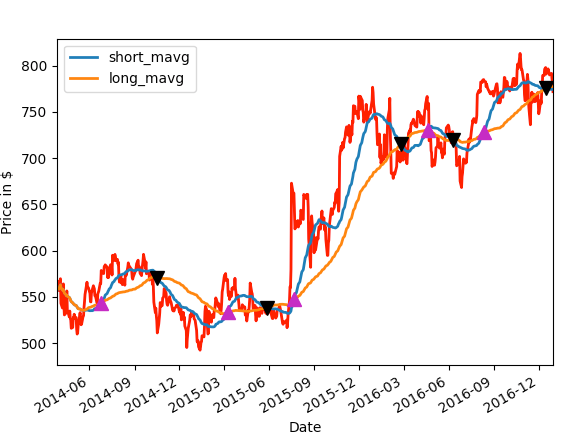
\includegraphics[width=90mm]{SMA_Google.png}
\caption{Simple Moving Average - "Golden Cross" Strategy applied to GOOG \label{overflow}}
\label{SMAfigure}
\end{figure}

\begin{figure}[h]
\centering
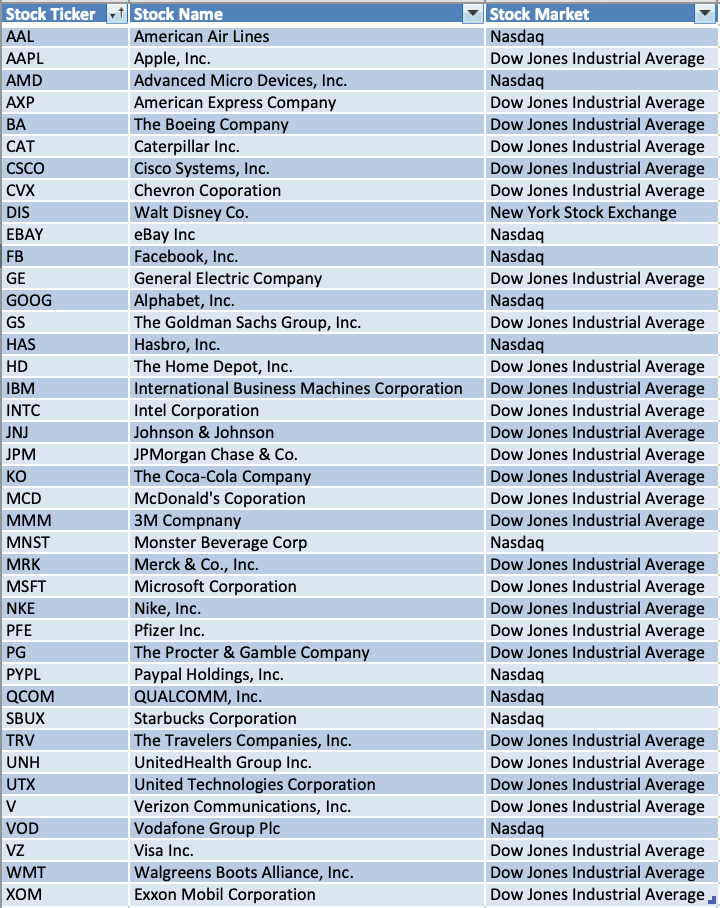
\includegraphics[width=85mm]{stock_table.png}
\caption{Table of stocks used in our study \label{overflow}}
\label{stocktable}
\end{figure}



\end{document}
